\documentclass[
  captions=tableheading,
  bibliography=totoc, 
  titepage=firstiscover,
]{scrartcl}

\usepackage{blindtext} %neuer input

\usepackage{longtable} % Tabellen über mehrere Seiten

\usepackage[utf8]{inputenc} %neuer input

\usepackage{scrhack}

\usepackage[aux]{rerunfilecheck} %Warnung falls nochmal kompiliert werden muss

\usepackage{fontspec} %Fonteinstellungen

\recalctypearea{}

\usepackage[main=ngerman]{babel} %deutsche Spracheinstellung

\usepackage{ragged2e} %neuer input

\usepackage{amsmath, nccmath}

\usepackage{amssymb} %viele mathe Symbole

\usepackage{mathtools} %Erweiterungen für amsmath


\DeclarePairedDelimiter{\abs}{\lvert}{\rvert}
\DeclarePairedDelimiter{\norm}{\lVert}{\rVert}

\DeclarePairedDelimiter{\bra}{\langle}{\rvert}
\DeclarePairedDelimiter{\ket}{\lvert}{\rangle}

\DeclarePairedDelimiterX{\braket}[2]{\langle}{\rangle}{
#1 \delimsize| #2
}

\NewDocumentCommand \dif {m}
{
\mathinner{\symup{d} #1}
}


\usepackage[
  math-style=ISO,
  bold-style=ISO,
  sans-style=italic,
  nabla=upright,
  partial=upright,
  warnings-off={
    mathtools-colon,
    mathtools-overbracket,
  },
]{unicode-math}

\setmathfont{Latin Modern Math}
\setmathfont{XITS Math}[range={scr, bfscr}]
\setmathfont{XITS Math}[range={cal, bfcal}, StylisticSet=1]


\usepackage[
  locale=DE,
  separate-uncertainty=true,
  per-mode=reciprocal,
  output-decimal-marker={,},
]{siunitx}

\usepackage[autostyle]{csquotes} %richtige Anführungszeichen

\usepackage{xfrac}

\usepackage{float}

\floatplacement{figure}{htbp}

\floatplacement{table}{htbp}

\usepackage[ %floats innerhalb einer section halten
  section,   %floats innerhalb er section halten
  below,     %unterhalb der Section aber auf der selben Seite ist ok
]{placeins}

\usepackage[
  labelfont=bf,
  font=small,
  width=0.9\textwidth,
]{caption}

\usepackage{subcaption} %subfigure, subtable, subref

\usepackage{graphicx}

\usepackage{grffile}

\usepackage{booktabs}

\usepackage{microtype} %Verbesserungen am Schriftbild

\usepackage[
backend=biber,
]{biblatex}

\addbibresource{../lit.bib}

\usepackage[ %Hyperlinks im Dokument
  german,
  unicode,
  pdfusetitle,
  pdfcreator={},
  pdfproducer={},
]{hyperref}

\usepackage{bookmark}

\usepackage[shortcuts]{extdash}

%\usepackage{warpcol}


\begin{document}
    \title{ATP Übungsblatt 4}
    \author{  
    Tobias Rücker\\
    \texorpdfstring{\href{mailto:tobias.ruecker@tu-dortmund.de}{tobias.ruecker@tu-dortmund.de}
    \and}{,} 
    Paul Störbrock\\
    \texorpdfstring{\href{mailto:paul.stoerbrock@tu-dortmund.de}{paul.stoerbrock@tu-dortmund.de}}{}
    }
\maketitle
\center{\Large Abgabegruppe: \textbf{Mittw. 10-12 Uhr}}
\thispagestyle{empty}

\newpage
\tableofcontents
\thispagestyle{empty}
\newpage

\setcounter{page}{1}


\section{Aufgabe 10}

    \begin{figure}[H]
        \centering
        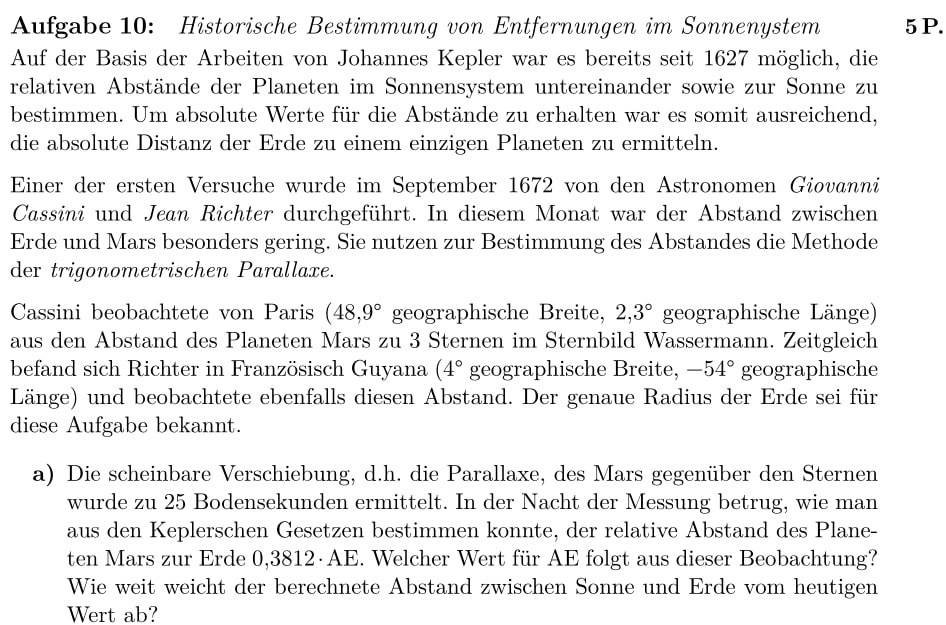
\includegraphics[width=\textwidth]{images/Aufgabe10.jpg}
        \label{fig:1}
    \end{figure}

    \flushleft{Um\;}\justifying die direkte Distanz $d$ der beiden Städte Paris ($P$) und Guyana($G$) zu bestimmen, wird das gleichschenklige 
    Dreieck Paris-Guyana-Erdmittelpunkt betrachtet. Die Schenkel sind hierbei der Erdradius $r_E$ und die Hypothenuse ist die direkte Distanz
    $d$. Dabei gilt es den von den Schenkeln aufgespanneten Winkel $\alpha$ zu bestimmen um auf $d$ schließen zu können.

    \flushleft{Paris\;}\justifying [Längengrad($L_1$): $\SI{2.3}{\degree}$, Breitengrad($B_1$): $\SI{48.9}{\degree}$] und Guyana [Längengrad($L_2$): $\SI{-54}{\degree}$, 
    Breitengrad($B_2$): $\SI{4}{\degree}$]
    \begin{align*}
        \alpha_x &= |L_1-L_2| = |\SI{2.3}{\degree}-(\SI{-54}{\degree})| = \SI{56.3}{\degree}\\
        \alpha_y &= |B_1-B_2| = |\SI{48.9}{\degree}-\SI{4}{\degree}| = \SI{44.9}{\degree}
        \intertext{\flushleft{Aus\;}\justifying $\alpha = \sqrt{\alpha_x^2+\alpha_y^2}$ folgt:
        }
        \alpha &= \SI{77.25}{\degree}
        \intertext{\flushleft{Aus\;}\justifying den obig genannten Verhältnis ergibt sich mit Pythagoras:
        }
        r_E^2 &= \left( \frac{d}{2} \right) +h 
        \intertext{\flushleft{Wobei\;}\justifying $h$ die Strecke zwischen Distanz $d$ und Erdmittelpunkt beschreibt.
        }
        \Rightarrow \cos\left( \frac{\alpha}{2} \right) &= \frac{h}{r_E}\\
        \Leftrightarrow h &= r_E \cos\left( \frac{\alpha}{2} \right)\\
        \left( \frac{d}{2} \right)^2 &= r_E^2 - r_E^2 \cos^2\left( \frac{\alpha}{2} \right)\\
        d &= 2r_E \sqrt{1-\cos^2\left( \frac{\alpha}{2} \right)}\\
        \Rightarrow d &= \SI{7491.562159}{\kilo\meter}
    \end{align*}
    \flushleft{Für\;}\justifying die Distanz $H$ zwischen Erde und Mars wird ein ähnliches gleichschenkliges Dreieck wie zuvor betrachtet,
    nur sind hier die Schenkel $e$ der Abstand zwischen Paris/Guyana und Mars. $d$ ist hier die selbe direkte Distanz zwischen Paris und Guyana,
    wobei der Winkel, der von den Schenkeln aufgespannt wird, hier $\beta$ ist. Daraus folgt analog zu der obigen Rechnung:
    \begin{align*}
        e^2 &= \left( \frac{d}{2} \right)^2 + e^2 \cos^2\left( \frac{\beta}{2} \right)\\
        e^2\left( 1-\cos\left( \frac{\beta}{2} \right) \right) &= \frac{d^2}{4}\\
        e &= \frac{d}{2\sqrt{1-\cos^2\left( \frac{\beta}{2} \right)}}\\
        \Rightarrow 0.3812 \text{AE} &= \frac{d}{2\sqrt{1-\cos^2\left( \frac{\beta}{2} \right)}}\\
        AE &= \frac{d}{2\cdot0.3812\sqrt{1-\cos^2\left( \frac{\beta}{2} \right)}}\\
        &= 8.812\cdot10^{20}\text{km}
    \end{align*}

\section{Aufgabe 11}

    \begin{figure}[H]
        \centering
        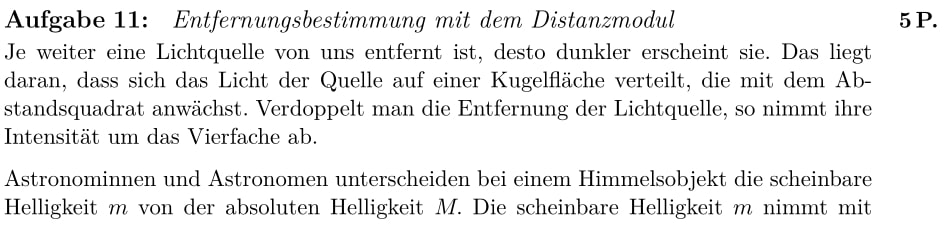
\includegraphics[width=\linewidth]{images/Aufgabe11_1.jpg}
        \label{fig:2}
    \end{figure}

    \begin{figure}[H]
        \centering
        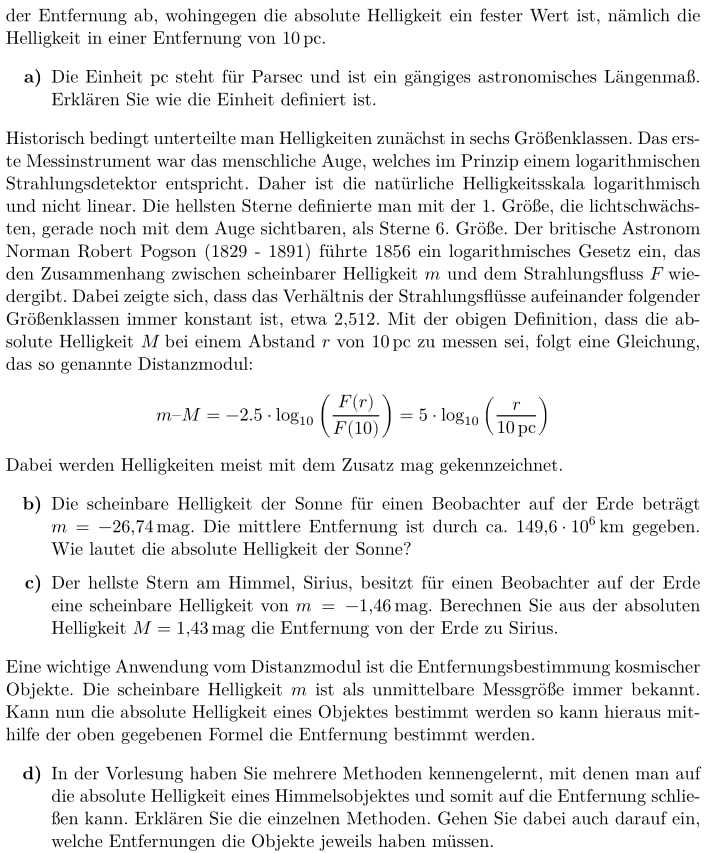
\includegraphics[width=\linewidth]{images/Aufgabe11_2.jpg}
        \label{fig:3}
    \end{figure}

    \begin{figure}[H]
        \centering
        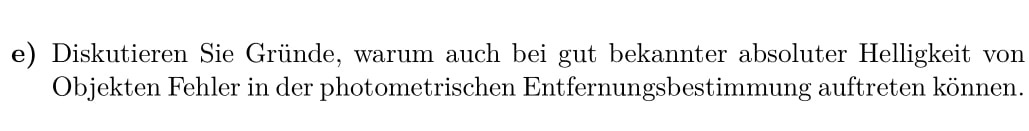
\includegraphics[width=\linewidth]{images/Aufgabe11_3.jpg}
        \label{fig:4}
    \end{figure}

    \subsection{a)}

    \flushleft{Ein\;}\justifying Parsec, oder Parallaxen Sekunde wird verwendet um die Distanz entfernter Lichtquellen im Universum 
    zu bestimmen. Dabei wird folgende Geometrie verwendet:

    \begin{figure}[H]
        \centering
        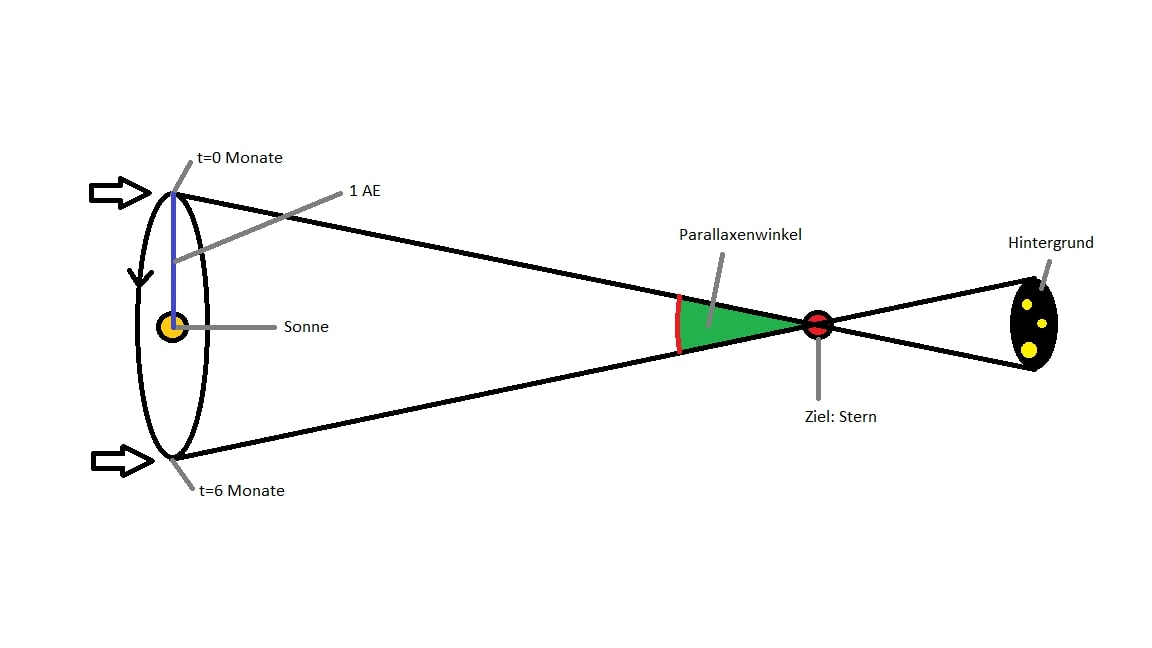
\includegraphics[width=\linewidth]{images/Parallaxe.jpg}
        \label{fig:5}
    \end{figure}

    \flushleft{Wird\;}\justifying der Stern in einem Abstand von sechs Monaten betrachtet, hat die Erde ihre Position um 2AE verändert. 
    Unter betrachtung des vergleichsweise statischen Hintergrund fällt nun auf, dass sich der gesuchte Stern um einen Winkel verschoben 
    hat. Dieser Winkel ist der Parallaxenwinkel und erlaubt es die Distanz zwischen Sonne und gesuchtem Stern zu ermitteln. 
    Ein Parsec ist die Distanz des Fluchtpunkts bei einem Parallaxenwinkel von einer Bogensekunde.

    \newpage
    \subsection{b)}

    \begin{align*}
        m-M &= 5 \cdot \log_{10}\left( \frac{1}{10pc} \right)\\
        \Leftrightarrow M &= m-5 \cdot \log_{10}\left( \frac{1}{10 \text{pc}} \right)
        \intertext{\flushleft{Werden\;}\justifying nun für $m=-26.74\,\text{mag}$ und $r=149.6\cdot10^6\SI{}{\kilo\meter}$ eingesetzt, ergibt sich
        } 
        M &= \text{\input{M.tex}}
    \end{align*}

    \subsection{c)}

    \begin{align*}
        m-M &= 5 \cdot \log_{10}\left( \frac{r}{10 \text{pc}} \right) \tag(*)\\
        &= 5\left(\log_{10}\left( \frac{r}{\text{pc}} \right)-\log_{10} \left( 10\right) \right)\\
        &= 5\left( \log_{10}\left(\frac{r}{\text{pc}}\right)-1 \right)\\
        \frac{m-M}{5}+1 &= \log_{10}\left(\frac{r}{\text{pc}}\right)\\
        \Rightarrow \frac{r}{\text{pc}} &= 10^{\left(\frac{m-M}{5}-1 \right)}\\
        r &= 10^{\frac{m-M}{5}+1} \text{pc}
        \intertext{\flushleft{Durch\;}\justifying einsetzen von $m=-1.46\,\text{mag}$ und $M=1.43\,\text{mag}$ ergibt sich:
        }
        r &= \text{\input{r.tex}}
    \end{align*}

    \subsection{d)}

    \flushleft{Die\;}\justifying Parallaxenmethode kann bei einzelnen Sternen sowie bei Sternenhaufen angewandt werden. Bei Sternhaufen
    wird die Sternstromparallaxe verwendet, wo der Konvergenzpunkt einzelner geeigneter Sterne betrachtet wird. Dazu muss die Relativbewegung
    der Erde, sowie die spektral Verschiebung berücksichtigt werden. Diese Methode kann Distanzen bis zu 130 Lj/40 pc bestimmen.

    \flushleft{Cepheiden\;}\justifying sind pulsierende Riesen, die über eine bestimmte Periode $T$ ihre Luminosität verändern. Die Luminosität
    hängt direkt mit der Länge der Periode zusammen, wodurch die wahre Leuchtkraft des Cepheids bestimmt werden kann. Mit bekannten Cepheiden
    (bekannte Luminosität und Periodendauer) kann mit $(*)$ auf den Abstand zu neuen Cepheiden geschlossen werden. Diese Methode kann Distanzen
    bis zu $10^7\,$Lj bestimmen.

    \flushleft{Die\;}\justifying Rotverschiebung ist ein Phenomen, welches der Ausdehnung des Raumes/des Universums zu verschulden ist. Durch
    die Expansion des Raumes wird ein relativistisch propagierendes Photon im Raum gedehnt, wodurch sich dessen Wellenlänge vergrößert. Bei 
    bekannten Spektren von Sternen oder Galaxien lässt sich diese Dehnung auf das ursprüngliche Spektrum zurückführen, wodurch die Distanz 
    errechnet werden kann. Die Genauigkeit schwankt jedoch, da dem Licht unterwegs viel im Weg stehen kann, dass sich auf den Dopplereffekt 
    auswirken kann. Demnach ist die Distanzmessung via Rotverschiebung nur bis auf ca. 100k Lj genau.

    \flushleft{Die\;}\justifying letzte Methode ist die der Standardkerzen. Obgleich selten, haben Supernovae des Typus Ia eine bekannte 
    Relation zwischen Luminosität und Breite der Lichtkurve. Hier tritt wieder die Rotverschiebung auf, welche zurückführt auf die Distanz. 
    Diese Messung ist bis zu $10^{10}\,$Lj genau. 

    \subsection{e)}

    \flushleft{Wie\;}\justifying bereits im Absatz der Rotverschiebung erklärt, kann dem Licht vieles im Weg stehen. Das Licht kann
    durch Gravitationsfelder gestreckt/gestaucht werden oder durch Gas/Staub an Intensität verlieren. Es ist zum Beispiel schwer bis 
    unmöglich Objekte auf der uns gegenüberliegender Seite der Milchstraße genau zu bestimmen, da zu viele Leuchtende Körper im Weg sind.
    Schwächer leuchtende Objekte können demnach vom Hintergrund "verschluckt" \;werden. 

\section{Aufgabe 12}

    \begin{figure}[H]
        \centering
        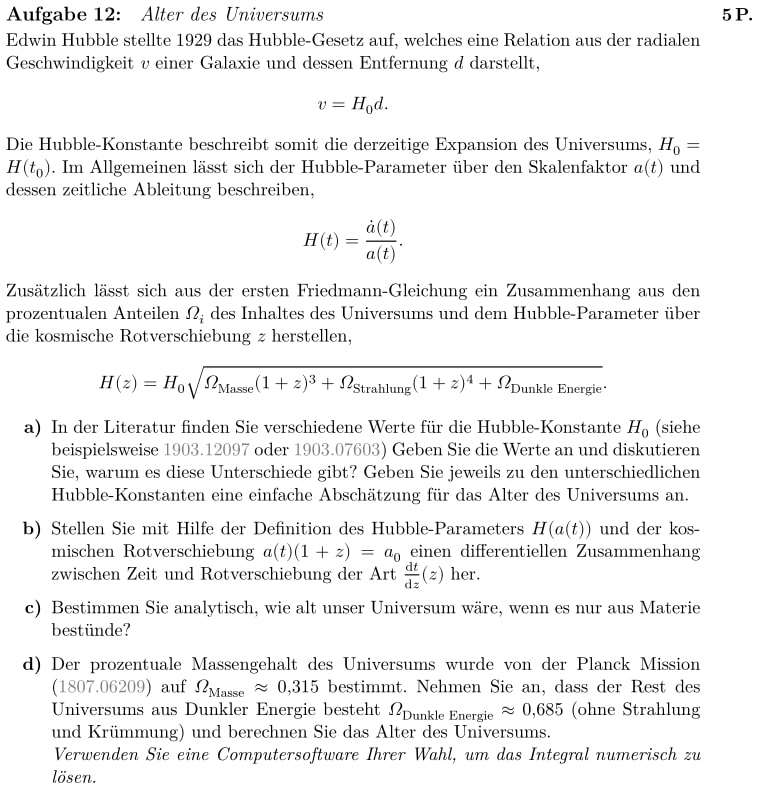
\includegraphics[width=\textwidth]{images/Aufgabe12.jpg}
        \label{fig:6}
    \end{figure}

    \subsection{a)}

    \subsection{b)}

    \subsection{c)}

    \subsection{d)}

\end{document}